%!TEX root = ../thesis.tex

% FIGURE: tau backgrounds
\begin{figure*}[p!]
  %\vspace{-3mm}
  \def\mybr{\\[-0.5pt]\phantom{.}\hspace{5.3mm}}
  \centerline{
    \subfloat[Genuine $\PGp^-$.]{ %$\PGt^\pm \to h^\pm \PGnGt$
      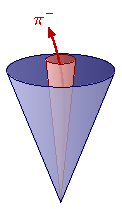
\includegraphics[width=0.145\linewidth,page=1]{fig/tau/jet_tau.pdf}} \hspace{1mm}
    \subfloat[Genuine\mybr$\PGp^- \PGp^0\PGp^0$.]{ %$\PGt^\pm \to h^\pm \PGp^0\PGp^0 \PGnGt$
      \includegraphics[width=0.145\linewidth,page=2]{fig/tau/jet_tau.pdf}} \hspace{1mm}
    \subfloat[Genuine\mybr$\PGp^+ \PGp^- \PGp^+ \PGp^0$.]{ %$\PGt^\pm \to h^\pm h^\pm h^\pm \PGp^0 \PGnGt$
      \includegraphics[width=0.145\linewidth,page=4]{fig/tau/jet_tau.pdf}} \hspace{1mm}
  %}\centerline{
    \subfloat[Isolated\mybr electron.]{
      \includegraphics[width=0.145\linewidth,page=5]{fig/tau/jet_tau.pdf}} \hspace{1mm}
    \subfloat[Isolated\mybr muon.]{
      \includegraphics[width=0.145\linewidth,page=6]{fig/tau/jet_tau.pdf}} %\hspace{0.4mm}
    \subfloat[Quark or\mybr gluon jet.]{
      \includegraphics[width=0.155\linewidth,page=7]{fig/tau/jet_tau.pdf}}
  }
  \caption{
Illustration of several hadronic decay modes of the $\PGt$ leptons (a-c) and their backgrounds (d-f).
Adapted from Ref.~\cite{tau_cones_fig}.
  } \label{fig:tau_jets}
  %\vspace{-3mm}
\end{figure*}
